\section{Auswertung}
\label{sec:Auswertung}

Im Folgenden werden alle Berechnungen in Python 3.7.1, unterstützt durch das
Paket NumPy \cite{numpy}, durchgeführt. Die Abbildungen werden mit matplotlib \cite{matplotlib} erstellt.

\subsection{Untersuchung des Spektrums}

Das Spektrum der Quelle ist in Abbildung \ref{fig:spektrum} dargestellt. Dort ist die Anzahl der gemessenen Ereignisse gegen die Nummer des Channels, in dem sich die Ereignisse befinden, aufgetragen.

\begin{figure}
  \centering
  \includegraphics[width=\textwidth]{build/spektrum.pdf}
  \caption{Spektrum der Caesium-Quelle.}
  \label{fig:spektrum}
\end{figure}

Bei der Betrachtung von links nach rechts sind im Spektrum zunächst beim ersten
Maximum die Rückstreulinie, danach das Compton-Kontinuum, daraufhin beim zweiten
Maximum die maximale Compton-Energie und anschließend der Photopeak zu sehen.

Die Rückstreulinie, markiert durch 1, entsteht dadurch, dass der Strahler in alle Richtungen strahlt und auch an den Bleiwänden Compton-gestreute Photonen in den Detektor gelangen können. Das Compton-Kontinuum (2) entsteht durch die Wechselwirkung der Gammaphotonen mit dem Szintillationsdetektor, wobei sie unter einem bestimmten Winkel gestreut werden und dabei Energie abgeben. Dieser Effekt wurde bereits in Kapitel \ref{subsec:theorie1} erläutert. Er findet nur bis zu einer bestimmten Energie statt, sodass sich die Compton-Kante (3) ergibt.
Der Photopeak, markiert durch 4, repräsentiert schließlich die tatsächliche Energie der Gammaphotonen
und beträgt \cite{energie}
\begin{equation*}
  E=\SI{661.7}{\kilo\eV} \,.
\end{equation*}
Der Peak lässt sich der Gammaenergie zuordnen, da diese diskret ist.

Die Zählrate für die Nullmessung ohne Würfel im Strahlengang kann zu
\begin{equation*}
  I_0=\SI{184.08(87)}{\per \second}
\end{equation*}
bestimmt werden.

\subsection{Untersuchung eines leeren Aluminiumgehäuses}

Zur Untersuchung des leeren Aluminiumgehäuses wurden für die in Abbildung \ref{fig:wuerfel1} dargestellten Projektionen die Zählraten gemessen.

\begin{figure}
  \centering
  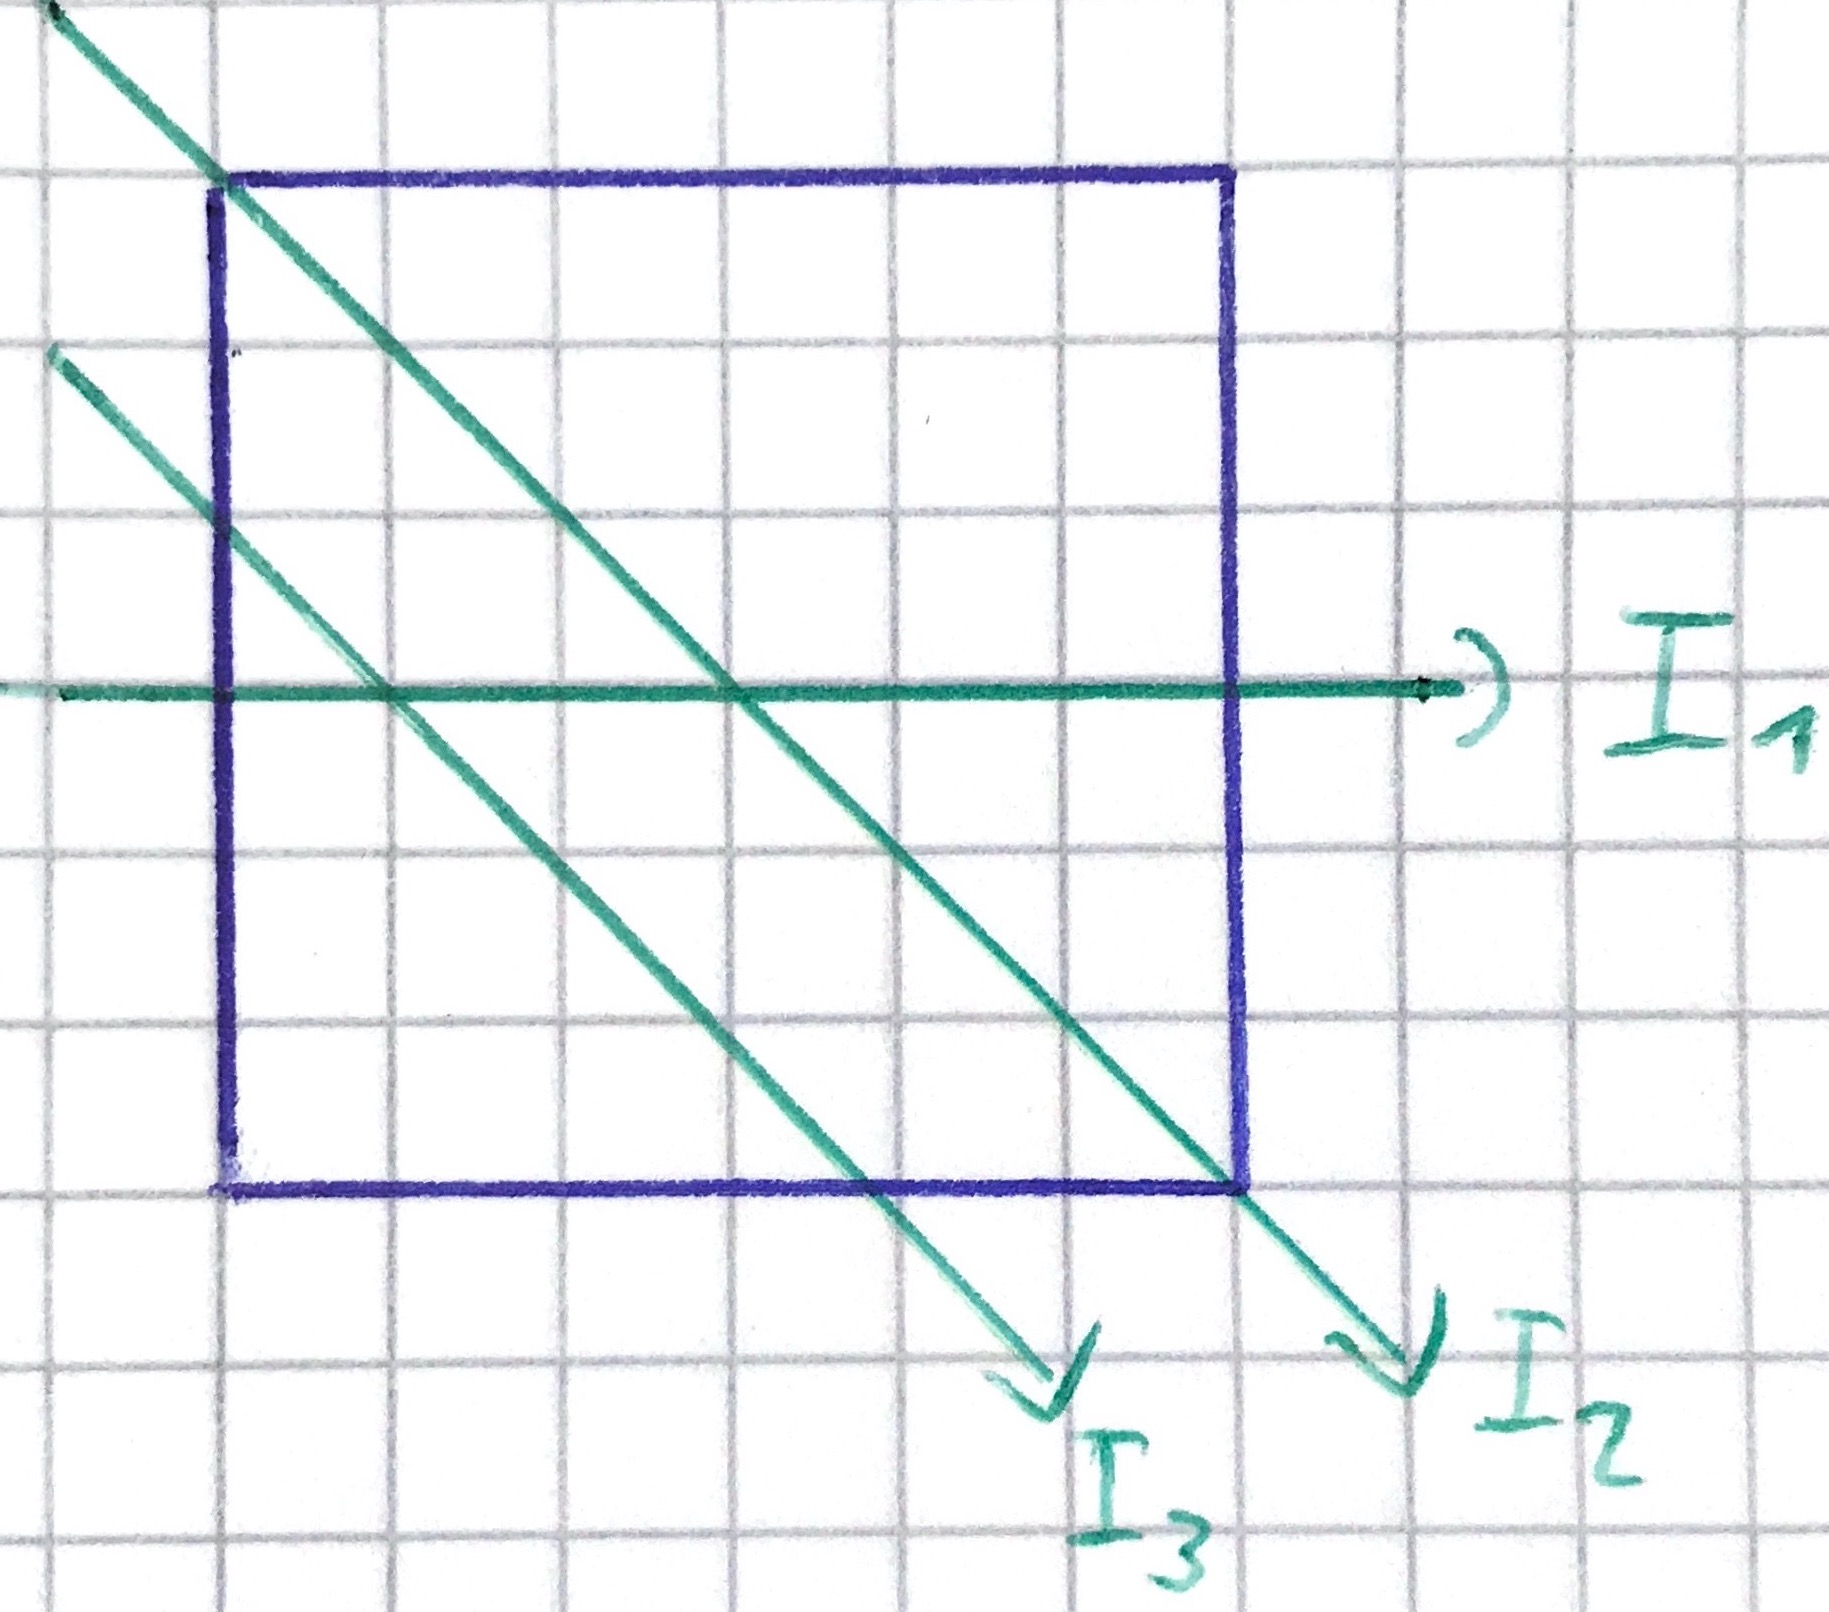
\includegraphics[width=0.5\textwidth]{images/wuerfel1.jpg}
  \caption{Skizze der gemessenen Projektionen für das reine Aluminiumgehäuse.}
  \label{fig:wuerfel1}
\end{figure}

Da alle folgenden Würfel ebenfalls ein Aluminiumgehäuse besitzen und die Absorption durch das Aluminiumgehäuse somit bei jedem Würfel auftritt, werden
diese Messungen als Nullmessungen für den jeweiligen Projektionstyp gewählt. Das bedeutet $I_{0,1}$ ist die Nullmessung für gerade Projektionen,  $I_{0,2}$ ist die Nullmessung für diagonale Projektionen durch eine Hauptdiagonale des Würfels
und $I_{0,3}$ ist die Nullmessung für diagonale Messungen durch eine Nebendiagonale des Würfels.

Es ergeben sich die Zählraten
\begin{align*}
  I_{0,1}&=\SI{171.83(135)}{\per\second} \,, \\
  I_{0,2}&=\SI{169.63(133)}{\per\second} \,, \\
  I_{0,3}&=\SI{158.78(133)}{\per\second} \,.
\end{align*}

\subsection{Bestimmung des Materials zweier homogener Würfel}
\label{subsec:wuerfel}
Zur Bestimmung des Materials zweier homogener Würfel werden die Zählraten für die
in Abbildung \ref{fig:wuerfel2} dargestellten Projektionen gemessen. Die gemessenen Werte befinden sich in Tabelle \ref{tab:wuerfel2}.

\begin{figure}
  \centering
  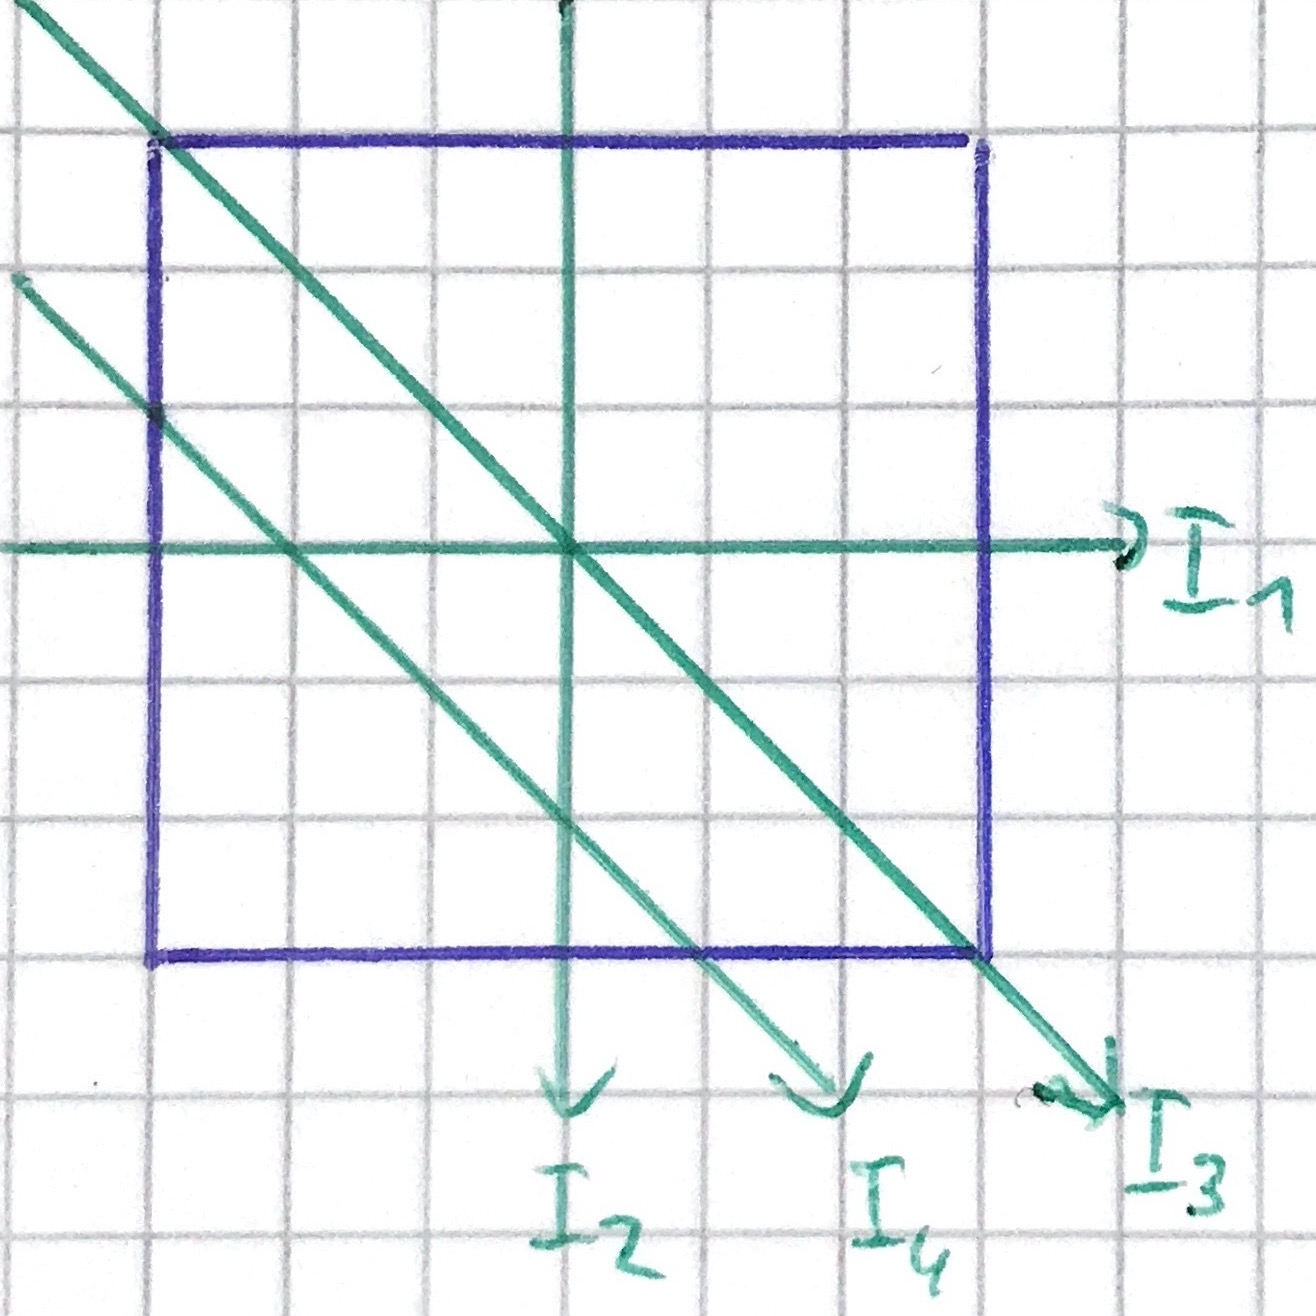
\includegraphics[width=0.5\textwidth]{images/wuerfel2.jpg}
  \caption{Skizze der gemessenen Projektionen für die homogenen Würfel.}
  \label{fig:wuerfel2}
\end{figure}

\begin{table}[htp]
	\begin{center}
    \caption{Messwerte und daraus berechnete Zählraten für die beiden homogenen Würfel.}
    \label{tab:wuerfel2}
		\begin{tabular}{c S[table-format=4.0,table-figures-uncertainty=2] S[table-format=2.2,table-figures-uncertainty=2] S[table-format=5.0,table-figures-uncertainty=3] S[table-format=3.2,table-figures-uncertainty=2]}
		\toprule
			{Projektion} & {$N_2$}  & {$I_2$/(1/s)}  & {$N_3$}  & {$I_3$/(1/s)}\\
			\midrule
			1 & 4981 \pm 80 & 27,67 \pm 0,44 & 20566 \pm 165 & 114,26 \pm 0,92\\
			2 & 4594 \pm 81 & 25,52 \pm 0,45 & 20670 \pm 167 & 114,83 \pm 0,93\\
			3 & 2906 \pm 62 & 16,14 \pm 0,34 & 17772 \pm 159 & 98,73  \pm 0,88\\
			4 & 4464 \pm 77 & 24,80 \pm 0,43 & 19603 \pm 166 & 108,91 \pm 0,92\\
		\bottomrule
		\end{tabular}
	\end{center}
\end{table}

Aus den gemessenen Zählraten kann der Absorptionskoeffizient über den Zusammenhang
\begin{equation}
  \mu_i=\frac{1}{l_i} \ln \left(\frac{I_{0,j}}{I_i} \right)
\end{equation}
bestimmt werden. Dabei ist $l_i$ die Strecke, die die Gammastrahlung durch den Würfel zurücklegt, $I_{0,j}$ die Nullzählrate für die entsprechende Art der Projektion und $I_i$ die Zählrate für die Projektion durch den Würfel. Der zugehörige Fehler kann mithilfe der Gauß'schen Fehlerfortpflanzung zu
\begin{equation}
  \Delta \mu_i=\sqrt{\left(  -\frac{\Delta I_i}{l_i I_i}\right)^2 \left( \frac{\Delta N_{0,j}}{l_j N_{0,j}}\right)^2}
\end{equation}
bestimmt werden. Die Ergebnisse sind in Tabelle \ref{tab:ergebnisse} dargestellt.

\begin{table}[htp]
	\begin{center}
    \caption{Berechnete Werte für die Absorptionskoeffizienten.}
    \label{tab:ergebnisse}
		\begin{tabular}{c S[table-format=0.3,table-figures-uncertainty=1] S[table-format=0.3,table-figures-uncertainty=1]}
		\toprule
		{Projektion} &{$\mu_2$/(1/cm)} & {$\mu_3$/(1/cm)}\\
			\midrule
			1 & 0,609 \pm 0,006 & 0,136 \pm 0,004\\
			2 & 0,636 \pm 0,006 & 0,134 \pm 0,004\\
			3 & 0,554 \pm 0,005 & 0,128 \pm 0,003\\
			4 & 0,656 \pm 0,007 & 0,133 \pm 0,004\\
		\bottomrule
		\end{tabular}
	\end{center}
\end{table}

Die Einzelergebnisse werden noch mit
\begin{align}
  \bar{\mu}&= \frac{1}{4} \sum_{i=1}^4 \mu_i \,
  %\Delta\bar{\mu}&=\sqrt{\frac{1}{12} \sum_{i=1}^4 (\bar{\mu}-\mu_i)^2}
\end{align}
gemittelt. Damit folgt für die gemittelten Absorptionskoeffizienten
\begin{align*}
  \bar{\mu}_2&= \SI{0.614(3)}{1\per \centi\metre}\,, \\
  \bar{\mu}_3&=\SI{0.133(2)}{1\per \centi\metre} \,.
\end{align*}
Damit können den Würfeln die Materialien Messing für Würfel 2 und
\ce{CH2O} für Würfel 3 zugeordnet werden. Die Abweichungen von den Literaturwerten (siehe Tabelle \ref{tab:dicke})
betragen $1{,}57\%$ und $14{,}75\%$.

\newpage
\subsection{Bestimmung der Materialien in einem zusammengesetzten Würfel}

Für den aus verschiedenen Materialien zusammengesetzten Würfel werden die Zählraten für die in Abbildung \ref{fig:wuerfel4} dargestellten Projektionen
gemessen. Die gemessenen Werte sind in Tabelle \ref{tab:wuerfel4} aufgeführt.

\begin{figure}
  \centering
  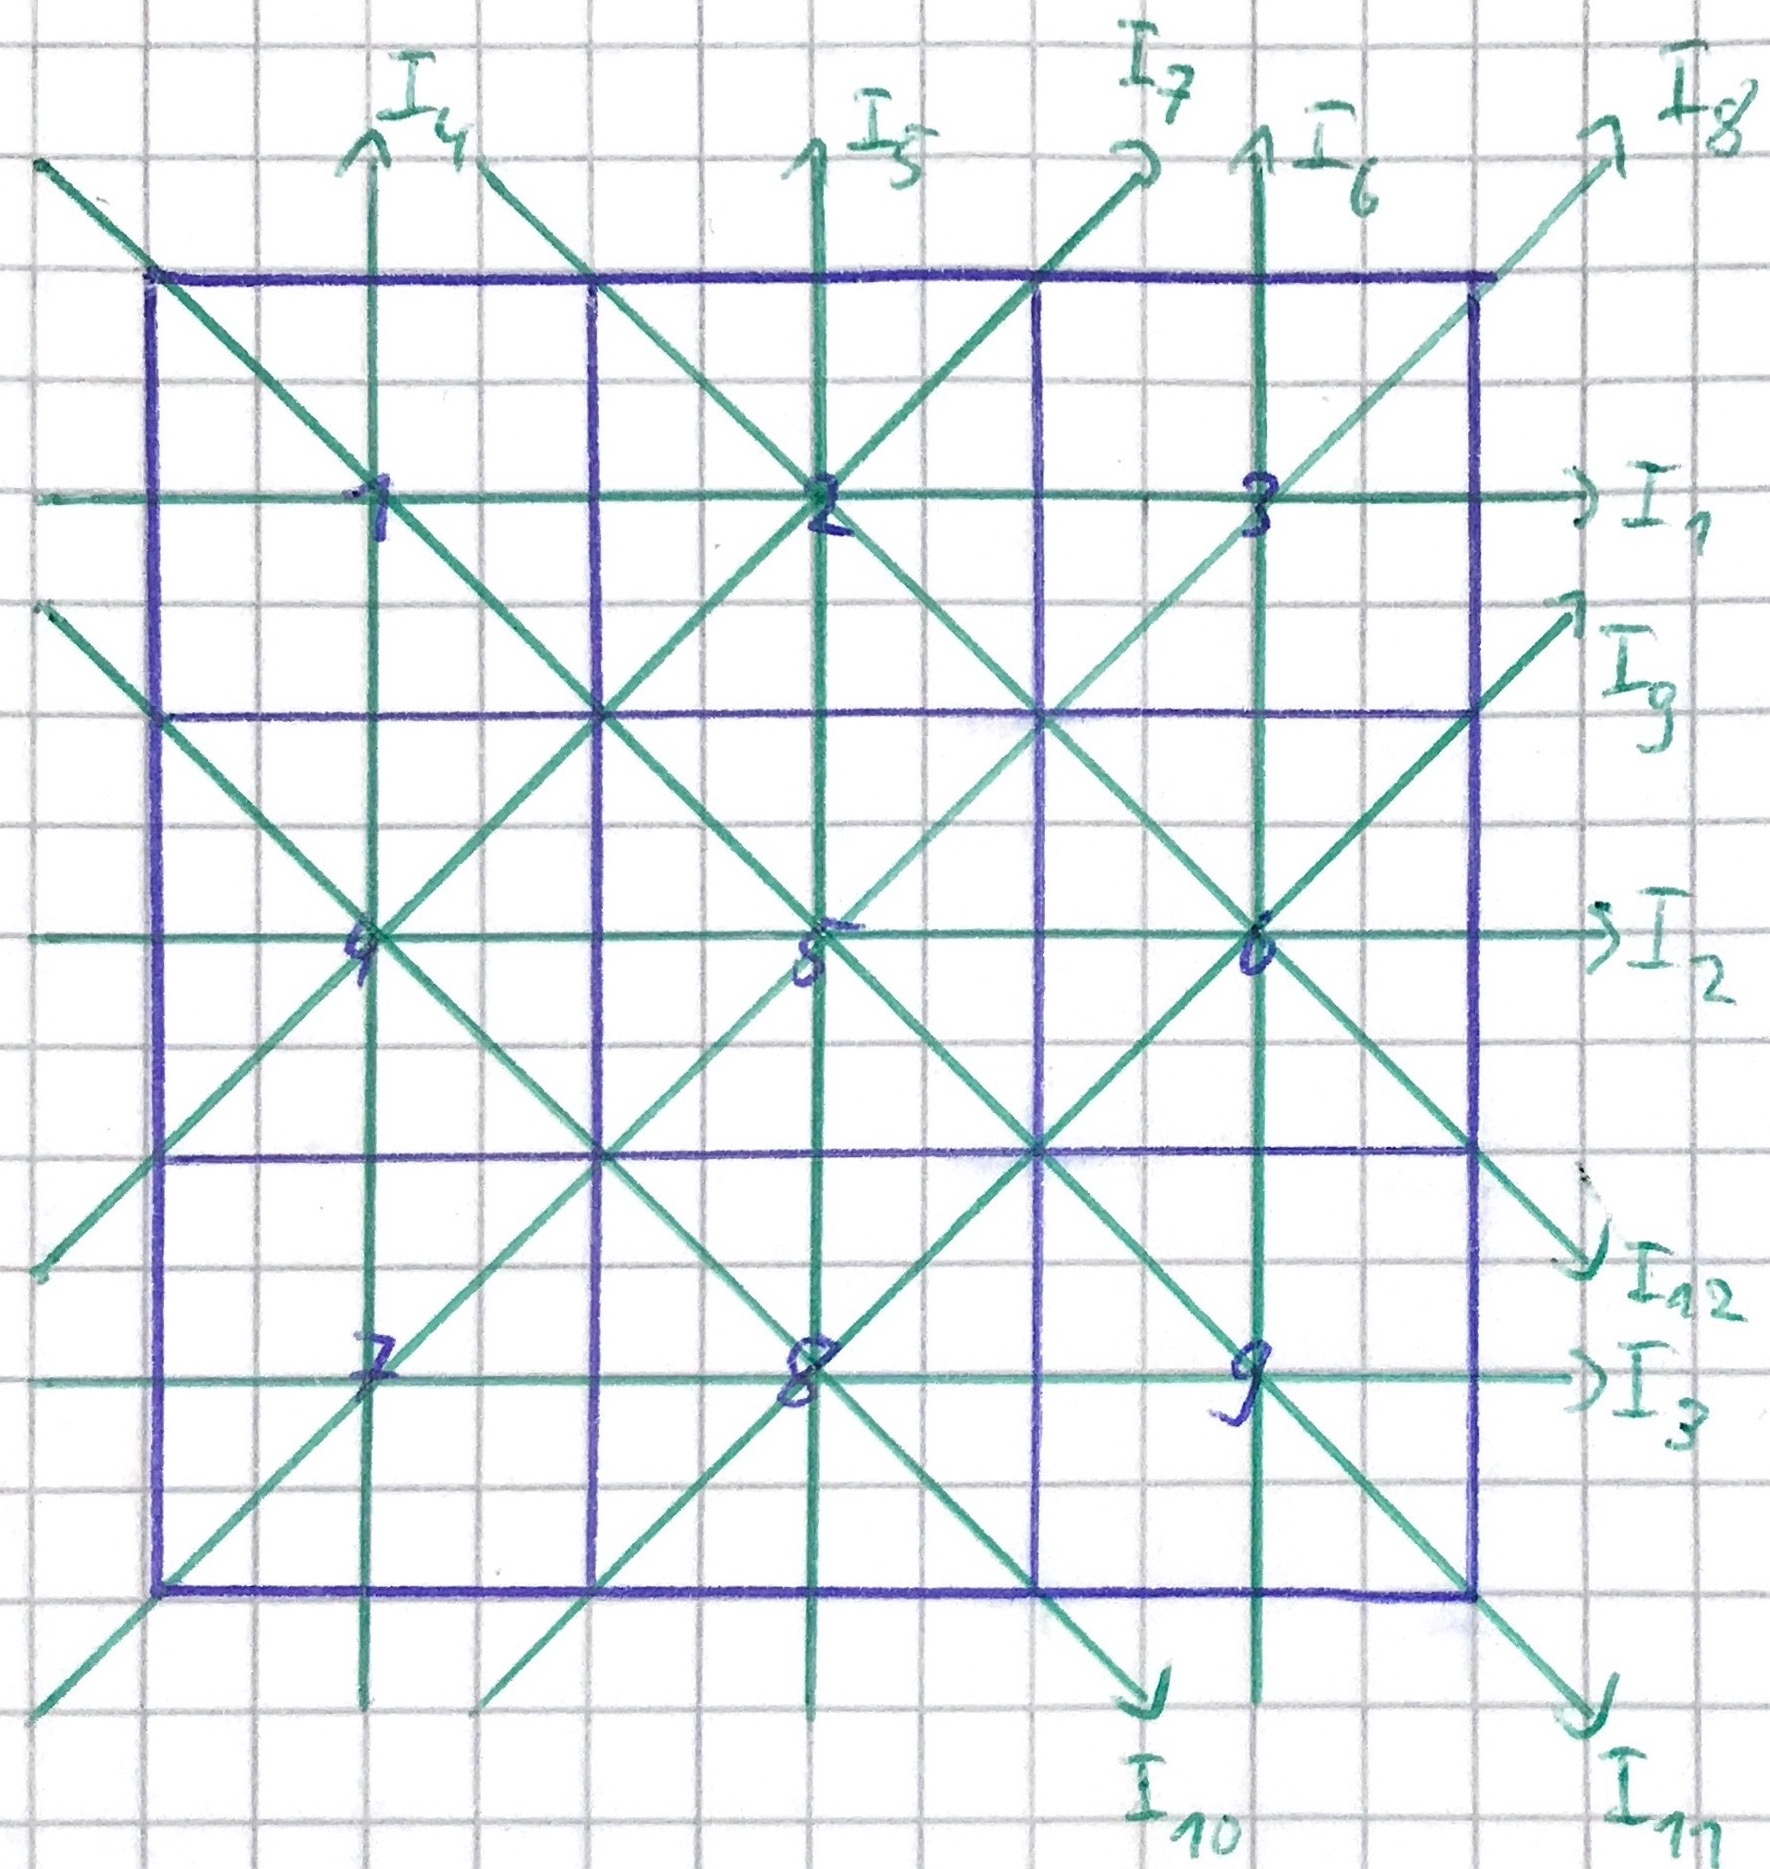
\includegraphics[width=\textwidth]{images/wuerfel4.jpg}
  \caption{Skizze der gemessenen Projektionen für den zusammengesetzten Würfel.}
  \label{fig:wuerfel4}
\end{figure}

\begin{table}[htp]
	\begin{center}
    \caption{Messwerte für die verschiedenen gemessenen Projektionen, sowie die daraus berechnete
    Zählrate.}
    \label{tab:wuerfel4}
		\begin{tabular}{c S[table-format=5.0,table-figures-uncertainty=3] S[table-format=3.2,table-figures-uncertainty=2]}
		\toprule
			{Projektion} &{$N_4$}  & {$I_4$/(1/s)} \\
			\midrule
			1 & 10544 \pm 134 &  58,58 \pm 0,74\\
			2 &  7572 \pm 133 &  42,07 \pm 0,74\\
			3 & 10487 \pm 134 &  58,26 \pm 0,74\\
			4 & 12869 \pm 131 &  71,49 \pm 0,73\\
			5 & 13396 \pm 130 &  74,42 \pm 0,72\\
			6 & 13328 \pm 131 &  74,04 \pm 0,73\\
			7 & 11420 \pm 137 &  63,44 \pm 0,76\\
			8 &  4565 \pm  79 &  25,36 \pm 0,44\\
			9 & 20651 \pm 162 & 114,73 \pm 0,90\\
			10 & 18717 \pm 154 & 103,98 \pm 0,86\\
			11 & 12013 \pm 124 &  66,74 \pm 0,69\\
			12 & 18251 \pm 152 & 101,39 \pm 0,84\\
		\bottomrule
		\end{tabular}
	\end{center}
\end{table}

Die zugehörige Matrix lautet dann
\begin{equation}
  A= d
  \left(
  \begin{array}{rrrrrrrrr}
    1 & 1 & 1 & 0 & 0 & 0 & 0 & 0 & 0 \\
    0 & 0 & 0 & 1 & 1 & 1 & 0 & 0 & 0 \\
    0 & 0 & 0 & 0 & 0 & 0 & 1 & 1 & 1 \\
    1 & 0 & 0 & 1 & 0 & 0 & 1 & 0 & 0 \\
    0 & 1 & 0 & 0 & 1 & 0 & 0 & 1 & 0 \\
    0 & 0 & 1 & 0 & 0 & 1 & 0 & 0 & 1 \\
    0 & \sqrt{2} & 0 & \sqrt{2} & 0 & 0 & 0 & 0 & 0 \\
    0 & 0 & \sqrt{2} & 0 & \sqrt{2} & 0 & \sqrt{2} & 0 & 0 \\
    0 & 0 & 0 & 0 & 0 & \sqrt{2} & 0 & \sqrt{2} & 0 \\
    0 & 0 & 0 & \sqrt{2} & 0 & 0 & 0 & \sqrt{2} & 0 \\
    \sqrt{2} & 0 & 0 & 0 & \sqrt{2} & 0 & 0 & 0 & \sqrt{2} \\
    0 & \sqrt{2} & 0 & 0 & 0 & \sqrt{2} & 0 & 0 & 0 \\
  \end{array}
  \right)\,.
\end{equation}

%Für die Intensitäten gilt
%\begin{equation*}
%  \vec{I}=   \left(
%    \begin{array}{r}
%      \ln\left(\frac{N_{0,1}}{N_{4,1}} \right) \\
%      \ln\left(\frac{N_{0,1}}{N_{4,2}} \right) \\
%      \ln\left(\frac{N_{0,1}}{N_{4,3}} \right) \\
%      \ln\left(\frac{N_{0,1}}{N_{4,4}} \right) \\
%      \ln\left(\frac{N_{0,1}}{N_{4,5}} \right) \\
%      \ln\left(\frac{N_{0,1}}{N_{4,6}} \right) \\
%      \ln\left(\frac{N_{0,2}}{N_{4,7}} \right) \\
%      \ln\left(\frac{N_{0,3}}{N_{4,8}} \right) \\
%      \ln\left(\frac{N_{0,2}}{N_{4,9}} \right) \\
%      \ln\left(\frac{N_{0,2}}{N_{4,10}} \right) \\
%      \ln\left(\frac{N_{0,3}}{N_{4,11}} \right) \\
%      \ln\left(\frac{N_{0,2}}{N_{4,12}} \right) \\
%    \end{array}
%    \right) \,.
%\end{equation*}
Der Intensitätsvektor $\vec{I}$ wird aus den Einträgen
\begin{equation*}
  \ln\left(\frac{N_{0,j}}{N_{4,i}}\right)
\end{equation*}
gebildet.

Nach Gleichung \eqref{eqn:mumatrix} kann dann der Vektor $\vec{\mu}$ zu
\begin{equation*}
  \vec{\mu}=
  \left(
      \begin{array}{r}
        \mu_1 \\
        \mu_2 \\
        \mu_3 \\
        \mu_4 \\
        \mu_5 \\
        \mu_6 \\
        \mu_7 \\
        \mu_8 \\
        \mu_9 \\
      \end{array}
      \right)=
  \left(
      \begin{array}{r}
        \SI{0.043(9)}{} \\
        \SI{0.298(7)}{} \\
        \SI{0.468(9)}{} \\
        \SI{0.406(7)}{} \\
        \SI{0.430(8)}{} \\
        \SI{0.205(7)}{} \\
        \SI{0.497(9)}{} \\
        \SI{0.080(6)}{} \\
        \SI{0.238(9)}{} \\
      \end{array}
      \right)
      \SI{}{\per\centi\meter}
\end{equation*}
berechnet werden. Die Fehler folgen aus dem Zusammenhang
\begin{equation}
  \sigma_{\mu_i} = \left(\sqrt{\frac{\symbf{\tilde{A}}^2 \sigma_{N}^2}{N^2} + \frac{\symbf{\tilde{A}}^{2} \sigma_{I_{0}}^2}{I_{0}^2}}\right)_i \\
  \text{mit}\:\: \symbf{\tilde{A}} = \left(\symbf{A^T} \cdot \symbf{A}\right)^{-1} \symbf{A^T}\,.
\end{equation}

So können die Materialien der kleinen Würfel, aus denen die Ebene des Würfels zusammengesetzt ist, bestimmt werden. Zunächst werden die Zuordnungen lediglich anhand des Vergleichs der berechneten Werte mit den Theoriewerten vorgenommen. Die
Zuordnungen und die Abweichungen der Werte von den Literaturwerten (siehe Tabelle \ref{tab:dicke}) ist in Tabelle \ref{tab:ergebnisse2} aufgeführt.
Die Literaturwerte für die Massenabschwächungskoeffizienten sind \cite{datenbank} entnommen, während die Dichte der Messinglegierung aus \cite{messing} abgelesen wird.
Es ist zu beachten, dass \ce{CH2O} nur das Monomer des Polymers Delrin ist, jedoch konnten auch nach gründlicher Recherche keine Werte für Delrin gefunden werden. Diese Ungenauigkeit sollte allerdings gegenüber den bereits vorhandenen Messungenauigkeiten vernachlässigbar sein.


\begin{table}[htp]
	\begin{center}
    \caption{Massenabschwächungskoeffizienten $\sigma$ in $\si{\centi\meter\squared\per\gram}$, Dichten in $\si{\gram\per\centi\meter\cubed}$ und Absorptionsskoeffizienten $\mu$ in $\si{\per\centi\meter}$ für die möglichen Materialien, aus denen die Elementarwürfel bestehen können.}
    \label{tab:dicke}
		\begin{tabular}{cccccccc}
		\toprule
			Material & $\sigma_{\text{photo}}$ & $\sigma_{\text{compton}}$ & $\sigma_{\text{ges}}$ & $\rho$ & $\mu_{\text{photo}}$ & $\mu_{\text{compton}}$ & $\mu_{\text{ges}}$\\
			\midrule
			Al & $\num{6.565e-5}$ & $\num{7.428e-2}$ & $\num{7.435e-2}$ & $\num{2.6989}$ & $\num{1.7718e-4}$ & $\num{0.2005}$ & $\num{0.2007}$\\
      Pb & $\num{4.337e-2}$ & $\num{6.015e-2}$ & $\num{1.035e-1}$ & $\num{11.35}$ & $\num{0.4922}$ & $\num{0.6827}$ & $\num{1.1747}$\\
      Fe & $\num{8.723e-4}$ & $\num{7.161e-2}$ & $\num{7.248e-2}$ & $\num{7.847}$ & $\num{6.8449e-3}$ & $\num{0.5619}$ & $\num{0.5688}$\\
      Messing & $\num{1.340e-3}$ & $\num{7.028e-2}$ & $\num{7.162e-2}$ & $\num{8.44}$ & $\num{1.1310e-2}$ & $\num{0.5932}$ & $\num{0.6045}$\\
      \ce{CH2O} & $\num{6.784e-6}$ & $\num{8.221e-2}$ & $\num{8.221e-2}$ & $\num{1.41}$ & $\num{9.5654e-6}$ & $\num{0.1159}$ & $\num{0.1159}$\\
		\bottomrule
		\end{tabular}
	\end{center}
\end{table}

\begin{table}[htp]
	\begin{center}
    \caption{Zuordnung der Materialien zu den Würfeln lediglich anhand des Vergleichs der Theoriewerte mit den berechneten Werten.}
    \label{tab:ergebnisse2}
		\begin{tabular}{ccc}
		\toprule
			{Würfel} & {Material}  & {Abweichung in \%} \\
			\midrule
			1 & \ce{CH2O} &   -62,90 \\
			2 & Al   &   48,95\\
			3 & Fe   &   -17,72\\
			4 & Fe   &   -28,62\\
			5 & Fe   &   -24,40\\
			6 & Al   &   2,46 \\
			7 & Fe   &   -12,62\\
			8 & \ce{CH2O} &   -30,97 \\
			9 & Al   &   18,96\\
		\bottomrule
		\end{tabular}
	\end{center}
\end{table}


Da aus der Versuchsanleitung bekannt ist, dass die Würfel nur aus den zwei in Kapitel
\ref{subsec:wuerfel} bestimmten Materialien Messing und \ce{CH2O} bestehen, können die
Materialien der Elementarwürfel noch genauer bestimmt werden. So ergeben sich die in
Tabelle \ref{tab:ergebnisse3} aufgeführten Zuordnungen.

\begin{table}[htp]
	\begin{center}
    \caption{Zuordnung der Materialien zu den Würfeln mit der zusätzlichen Einschränkung auf die Materialien Messing und \ce{CH2O}.}
    \label{tab:ergebnisse3}
		\begin{tabular}{ccc}
		\toprule
			{Würfel} & {Material}  & {Abweichung in \%} \\
			\midrule
			1 & \ce{CH2O}      &   -62,90 \\
			2 & CH20      &   157,12\\
			3 & Messing   &   -22,58\\
			4 & Messing   &   -32,84\\
			5 & Messing   &   -28,87\\
			6 & CH20      &   76,88 \\
			7 & Messing   &   -17,78\\
			8 & \ce{CH2O}      &   -30,97 \\
			9 & CH20      &   105,35\\
		\bottomrule
		\end{tabular}
	\end{center}
\end{table}
